\published{Journal of Seismic Exploration, 23, no. 4, 303-312, (2014)}

\title{Time-frequency analysis of seismic data using synchrosqueezing wavelet transform}
\renewcommand{\thefootnote}{\fnsymbol{footnote}}

\author{Yangkang Chen\footnotemark[1], Tingting Liu\footnotemark[2], Xiaohong Chen\footnotemark[2], Jingye Li\footnotemark[2] and Erying Wang\footnotemark[3]}

\address{
\footnotemark[1]Bureau of Economic Geology \\
John A. and Katherine G. Jackson School of Geosciences \\
The University of Texas at Austin \\
University Station, Box X \\
Austin, TX 78713-8924 \\
ykchen@utexas.edu\\
+1-5125478899 \\
ykchen@utexas.edu\\

\footnotemark[2] State Key Laboratory of Petroleum Resources and Prospecting \\
China University of Petroleum \\
Fuxue Road 18th\\
Beijing, China, 102200 \\
liutingjiy@126.com \\

\footnotemark[3] PetroChina Changqing Oilfield Company \\
Weiyang Road 35th \\
Xi'an,Shaanxi Province,China \\ 
wswey2008@126.com\\
}

\lefthead{Chen et al.}
\righthead{Time-frequency analysis using SSWT}

\maketitle

\begin{abstract}
Time-frequency (TF) decomposition is used for characterizing the non-stationary relation between time and instantaneous frequency, which is very important in the processing and interpretation of seismic data. The conventional time-frequency analysis approaches suffer from the contradiction between time resolution and frequency resolution. A new time-frequency analysis approach is proposed based on the synchrosqueezing wavelet transform (SSWT). The SSWT is an empirical-mode-decomposition-like tool but uses a different approach in constructing the components. With the help of the synchrosqueezing techniques, the SSWT can obtain obvious higher time and frequency resolution. Synthetic examples show that the SSWT based TF analysis can exactly capture the variable frequency components. Field data tests show the potential of the proposed approach in detecting anomalies of high-frequency attenuation and detecting the deep-layer weak signal.
\end{abstract}

\section{Keywords}
Time-frequency analysis, synchrosqueezing wavelet transform, low-frequency anomalies, deep-layer weak signal


\section{Introduction}
Time-frequency (TF) analysis solves the problems of identifying and quantifying the oscillatory components presented in the signal, % \cite[]{iatsenko2013}}, 
which has been exclusively utilized by the field of exploration geophysics over the past two decades \cite[]{partyka1999,castagna2003,reine2009,guochang20112}. One of the most common use of TF analysis is that deeper channels are usually stronger at lower frequency and the shallower flank of the channel has stronger amplitudes at higher frequencies. In addition, TF analysis can be used to estimating attenuation, pore-pressure prediction, and seismic unconformities, and some implementation of seismic chronostratigraphy \cite[]{tengfei2013}. Many approaches have been proposed for TF analysis, such as wavelet transform (WT), shot-time Fourier transform (STFT), Wigner-Ville distribution (WVD), S transform and recently proposed local attributes based TF \cite[]{guochang20112}. All of the mentioned approaches have their own advantages, however, they all have limited resolution either in time or in frequency.

The empirical mode decomposition (EMD) \cite[]{emd} algorithm can separate a signal into locally-constant frequency components, and have been shown to have a high resolution both in time and frequency with some types of extensions, like ensemble empirical mode decomposition (EEMD) and complete ensemble empirical mode decomposition (CEEMD). However, the EMD algorithm is still remaining heuristic because of the lack of mathematical support. The newly proposed synchrosqueezing wavelet transform (SSWT) capture the flavor and philosophy of the EMD approach, but with a mathematical way in constructing the components \cite[]{daubechies2011}. Because of the high-resolution property of SSWT, it is becoming more and more popular for characterizing non-stationary property in signal analysis field recently. In the exploration field, SSWT has been successfully used for removing ground rolls \cite[]{shang2013}. In this abstract, we use one benchmark non-stationary synthetic model for showing SSWT's high resolution both in time and frequency compared with other two robust TF decomposition approaches. We also applied SSWT onto two field data examples and show its potential in detecting anomalies of high-frequency attenuation and detecting deep-layer weak signal.  

\section{Synchrosqueezing wavelet transform}
The well-known continuous wavelet transform is defined by:
\begin{equation}
\label{eq:w1t}
W_x(a,t)=\int_{-\infty}^{\infty}x(\tau)a^{-1/2}\psi^*\left(\frac{\tau-t}{a}\right)d\tau,
\end{equation}
where $\psi(t)$ is the chosen mother wavelet, $\psi^*$ denotes the complex conjugate of $\psi$. The instantaneous frequency of $w_x(a,t)$ for signal $x(t)$ can be got by:
\begin{equation}
\label{eq:instf}
w_x(a,t) = -i(W_x(a,t))^{-1}\frac{\partial}{\partial t}W_x(a,t).
\end{equation}
The synchrosqueezed transform $T_x(w,t)$ can be determined only at the centers $w_l$ of the successive bins $[w_l-\frac{1}{2}\Delta w,w_l+\frac{1}{2}\Delta w]$, with $w_l-w_{l-1}=\Delta w$, by summing
different contributions \cite[]{daubechies2011}:
\begin{equation}
\label{eq:sswt}
T_x(w_l,t)=(\Delta w)^{-1} \sum_{a_k:|w(a_k,t)-w_l|\le \Delta w/2}^{} W_x(a_k,t)a_k^{-3/2}(\Delta a)_k.
\end{equation}
The SSWT is invertible and the original signal can be obtained by:
\begin{equation}
\label{eq:sswt}
\begin{split}
x(t) &= \mathcal{Re}\left[C_{\psi}^{-1}\int_{0}^{\infty}W_x(a,t)a^{-3/2}da\right] \\
	 &=\mathcal{Re}\left[C_{\psi}^{-1}\sum_{k}(a_k,t)a_k^{-3/2}(\Delta a)_k\right] \\
     &=\mathcal{Re}\left[C_{\psi}^{-1}\sum_{l}T_x(w_l,t)(\Delta w)\right].
\end{split}
\end{equation}

%\section{Synsqueezing wavelet transform}
\section{Examples}
\subsection{Benchmark synthetic example}
We first use a synthetic example to demonstrate the SSWT's high resolution both in time and frequency. The synthetic data is borrowed from \cite{guochang20112}. It is composed of three constant-frequency components and two spikes, as shown in Figure \ref{fig:s-0}. We compare the TF analysis result of the SSWT with that of the S transform and local-attributes based TF analysis.  %Here we don't compare the SSWT with conventional wavelet-based TF because \cite{shang2013} has already done that. 
The differences among the three TF analysis approaches are obvious. The SSWT exactly capture the three constant-frequency component and get a higher time resolution for the two spikes compared with the other two approaches. In the next part, we apply the SSWT to two field datasets to show its application in detecting low-frequency anomalies and deep-layer weak signal.

%\subsection{Field examples}
\subsection{Field examples}
The first field data (Figure \ref{fig:data}) is a land seismic survey used previously by \cite[]{fomel20132}. We extract two frequency slices (30 Hz and 60 Hz) from the TF decomposed result and show them in Figures \ref{fig:lowf} and \ref{fig:higf}. It's obvious that the high-frequency slice has some anomalies pointed out by the labels, which may comes from the high-frequency attenuation because of the trapped oil \& gas. The results are consistent from that found by \cite{fomel20132} using a different technique. The TF cube of the real data corresponding to three different TF analysis approaches are shown in Figure \ref{fig:timefreq-st,timefreq,pp-tfsswt}. The TF map of the S transform seems blurs together. While the local attributes based TF analysis can have good time resolution, the SSWT can get a better result.
%TF map with high temporal and frequency resolution. 
The deep-layer of the TF cube show coherent frequency components, indicating the %layered shape, which may corresponds to the deep-layer 
potential week signal which can not be sensed visually or by the other two TF analysis approaches. The detection of deep-layer week signal is significant because these weak signals usually indicate the existence of layers that has obvious impedance difference compared with their overburden layers. Especially when the detected signals are mainly existing in the low frequency band, the detection will indicate the existence of residual oil\&gas traps.


\begin{figure}[htb!]
  \centering
  \subfigure[]{\includegraphics[width=\columnwidth,height=0.320\columnwidth]{gch1/Fig/s-0}
    \label{fig:s-0}}
  \subfigure[]{\includegraphics[width=\columnwidth,height=0.320\columnwidth]{gch1/Fig/st-0}
    \label{fig:st-0}}
  \subfigure[]{\includegraphics[width=\columnwidth,height=0.320\columnwidth]{gch1/Fig/proj-0}
    \label{fig:proj-0}}
  \subfigure[]{\includegraphics[width=\columnwidth,height=0.320\columnwidth]{gch1/Fig/gch1-tfsswt}
    \label{fig:gch1-tfsswt}}
	\caption{(a) Synthetic signal with three constant-frequency components and two spikes, borrowed from \cite[]{guochang20112}. (b) Time-frequency map of the S transform. (c) Time-frequency map using local attributes. (d) Time-frequency map using the synchrosqueezing wavelet transform.}
   \label{fig:s-0,st-0,proj-0,gch1-tfsswt}
\end{figure}


The second field data example is a post-stack field data set, which is also used in the literature by \cite{guochang20112}. The data is shown in Figure \ref{fig:data2}. In this example, we extract three constant-frequency slices corresponding to 20Hz, 40Hz, and 60 Hz, using three different TF decomposition approaches: TF decomposition using the S transform, TF decomposition using local attributes and TF decomposition using the SSWT. We also extract a time-frequency spectral map for the 80th trace in the field data shown in Figure \ref{fig:data2}. All the constant-frequency slices and TF spectral map are shown in Figure \ref{fig:s1-0,s2-0,s3-0,tf-s,l1-0,l2-0,l3-0,tf-l,ss1-0,ss2-0,ss3-0,tf-ss}.

From the constant-frequency slices shown in Figure \ref{fig:s1-0,s2-0,s3-0,tf-s,l1-0,l2-0,l3-0,tf-l,ss1-0,ss2-0,ss3-0,tf-ss}, we can observe that the S transform has the lowest time resolution, followed by the local-attributes related TF decomposition. The constant-frequency slices and the TF spectral map from the SSWT both show that the TF decomposed results have the largest resolution both in time and frequency. From the TF spectral map, the S transform has a slightly lower frequency resolution. By the SSWT based TF decomposition, we can detect several low-frequency anomalies. In this example, we just emphasize four clearest anormalies, and point out them by four frame boxes with different colors. To better illustrate the result, let us first focus on Figure \ref{fig:ss1}. The four frame boxes pointed out four strong-amplitude areas, which do not show in its corresponding higher-frequency slices. Thus, these four anomalies may indicate potential oil\&gas traps with high probability. Even though from the constant-frequency slices using other two approaches have more or less some anomalies, these anomalies are not very easy to detect. Some highly-potential sweet spots have been lost by using the other two approaches, e.g., area pointed out by the four frame boxes. The best strategy for implementing the SSWT based TF decomposition onto the interpretation for subsurface phenomenons is to combine the SSWT based TF decomposition with the conventional approaches. While the SSWT based TF decomposition can point out the potential anomalies with high fidelity, a more convincing conclusion can be obtained by considering the results from the other approaches.

\section{Conclusions}
We have proposed a new TF analysis approach for seismic data using the synchrosqueezing wavelet transform. The proposed approach can achieve higher resolution both in time and frequency compared with the S transform and the local-attributes based TF decomposition. Numerical examples show that the SSWT can capture the variable-frequency components embedded in the non-stationary signal exactly. We show the potential of the SSWT %based time-frequency decomposition 
in detecting anomalies of high-frequency attenuation, which is crucial for finding  oil \& gas traps. Field data  tests also show that the proposed TF analysis approach can also help to detect deep-layer weak signal that is usually smeared in seismic data, which in turns can help to find deserted residual oil \& gas.

\begin{figure}[htb!]
  \centering
  \subfigure[]{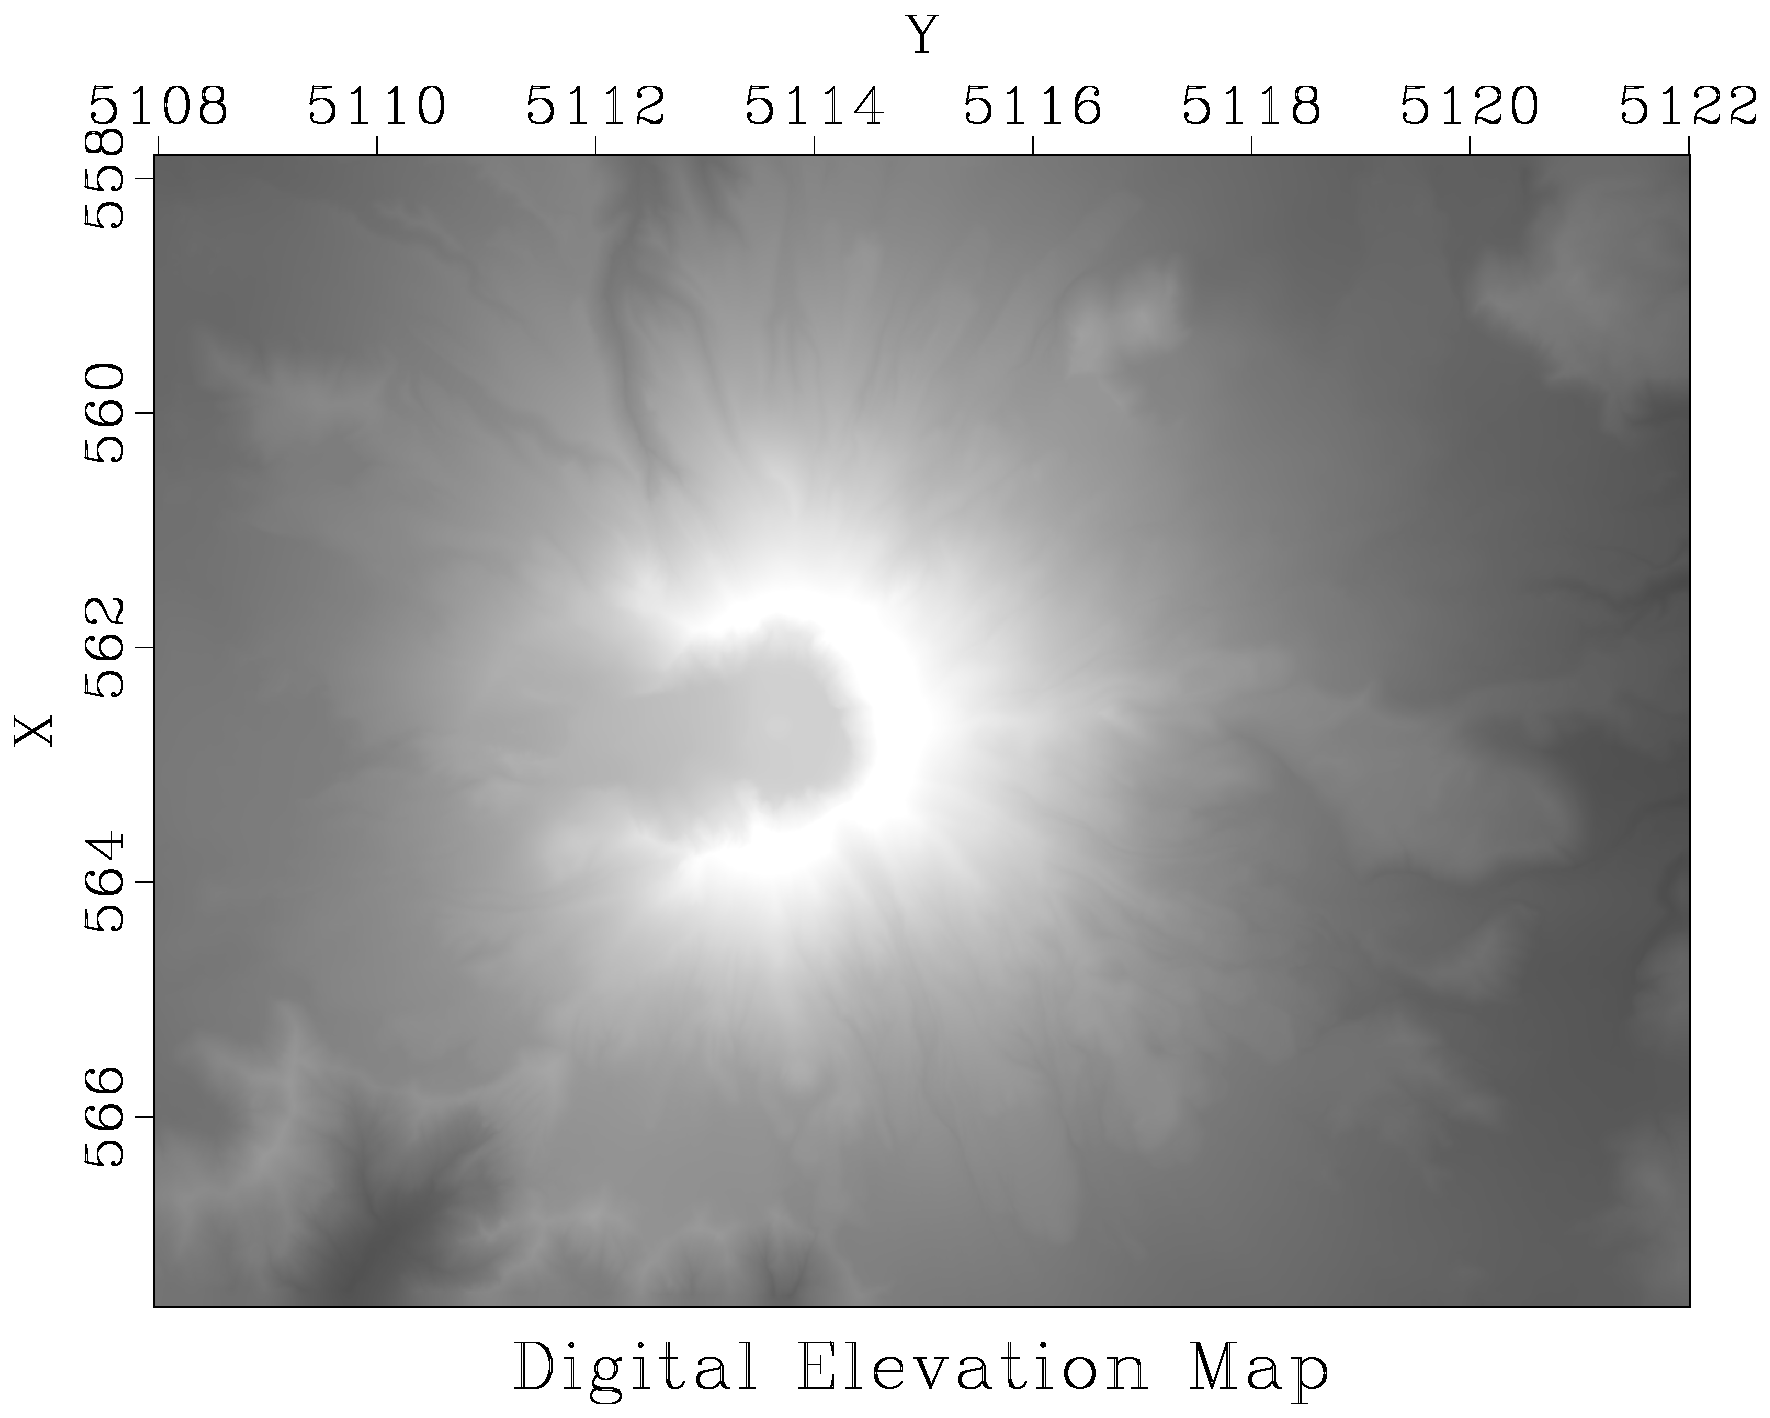
\includegraphics[width=0.8\columnwidth,height=0.45\columnwidth]{pp/Fig/data}
    \label{fig:data}}
  \subfigure[]{\includegraphics[width=0.8\columnwidth,height=0.45\columnwidth]{pp/Fig/lowf}
    \label{fig:lowf}}
  \subfigure[]{\includegraphics[width=0.8\columnwidth,height=0.45\columnwidth]{pp/Fig/higf}
    \label{fig:higf}}
	\caption{(a) Input data. (a) Frequency slice corresponding to 30 Hz. (b) Frequency slice corresponding to 60 Hz.}
   \label{fig:data,lowf,higf}
\end{figure}

\begin{figure}[htb!]
  \centering
  \subfigure[]{\includegraphics[width=0.8\columnwidth,height=0.45\columnwidth]{pp/Fig/timefreq-st}
    \label{fig:timefreq-st}}
  \subfigure[]{\includegraphics[width=0.8\columnwidth,height=0.45\columnwidth]{pp/Fig/timefreq}
    \label{fig:timefreq}}
  \subfigure[]{\includegraphics[width=0.8\columnwidth,height=0.45\columnwidth]{pp/Fig/pp-tfsswt}
    \label{fig:pp-tfsswt}}
	\caption{(a) Time-frequency map of the S transform. (b) Time-frequency map using local attributes. (c) Time-frequency map using the synchrosqueezing wavelet transform.}
   \label{fig:timefreq-st,timefreq,pp-tfsswt}
\end{figure}

\begin{figure}[htb!]
  \centering
  \includegraphics[width=\columnwidth,height=0.55\columnwidth]{lowf/Fig/old-1}
	\caption{Field data example for detecting low frequency anomalies.}
   \label{fig:data2}
\end{figure}

\section{Acknowledgments}
We would like to thank Guochang Liu for making the benchmark synthetic example publicly available, and developers of Madagascar software package for providing corresponding codes for testing the algorithms and preparing the figures.

\begin{figure}[htb!]
  \centering
  \subfigure[]{\includegraphics[width=0.25\columnwidth,height=0.320\columnwidth]{lowf/Fig/s1-0}
    \label{fig:s1}}
  \subfigure[]{\includegraphics[width=0.25\columnwidth,height=0.320\columnwidth]{lowf/Fig/s2-0}
    \label{fig:s2}}
  \subfigure[]{\includegraphics[width=0.25\columnwidth,height=0.320\columnwidth]{lowf/Fig/s3-0}
    \label{fig:s3}}
  \subfigure[]{\includegraphics[width=0.18\columnwidth,height=0.320\columnwidth]{lowf/Fig/tf-s}
    \label{fig:tf-s}}
  \subfigure[]{\includegraphics[width=0.25\columnwidth,height=0.320\columnwidth]{lowf/Fig/l1-0}
    \label{fig:l1}}
  \subfigure[]{\includegraphics[width=0.25\columnwidth,height=0.320\columnwidth]{lowf/Fig/l2-0}
    \label{fig:l2}}
  \subfigure[]{\includegraphics[width=0.25\columnwidth,height=0.320\columnwidth]{lowf/Fig/l3-0}
    \label{fig:l3}}
  \subfigure[]{\includegraphics[width=0.18\columnwidth,height=0.320\columnwidth]{lowf/Fig/tf-l}
    \label{fig:tf-l}}
  \subfigure[]{\includegraphics[width=0.25\columnwidth,height=0.320\columnwidth]{lowf/Fig/ss1-0}
    \label{fig:ss1}}
  \subfigure[]{\includegraphics[width=0.25\columnwidth,height=0.320\columnwidth]{lowf/Fig/ss2-0}
    \label{fig:ss2}}
  \subfigure[]{\includegraphics[width=0.25\columnwidth,height=0.320\columnwidth]{lowf/Fig/ss3-0}
    \label{fig:ss3}}
  \subfigure[]{\includegraphics[width=0.18\columnwidth,height=0.320\columnwidth]{lowf/Fig/tf-ss}
    \label{fig:tf-ss}}

	\caption{(a)-(c) Frequency slices of 20Hz, 40Hz, and 60 Hz, using the S transform. (d) Time-frequency spectral map using the S transform for 80th trace of the seismic profile shown in Figure \ref{fig:data2}. (e)-(g) Frequency slices of 20Hz, 40Hz, and 60 Hz, using the local-attributes related TF decomposition. (h) Time-frequency spectral map using the local-attributes related TF decomposition for 80th trace of the seismic profile shown in Figure \ref{fig:data2}.  (i)-(k) Frequency slices of 20Hz, 40Hz, and 60 Hz, using the SSWT. (l) Time-frequency spectral map using the SSWT for 80th trace of the seismic profile shown in Figure \ref{fig:data2}. }
   \label{fig:s1-0,s2-0,s3-0,tf-s,l1-0,l2-0,l3-0,tf-l,ss1-0,ss2-0,ss3-0,tf-ss}
\end{figure}

\bibliographystyle{seg}
\bibliography{synwav}







